%!TEX root = main.tex
\section{Grundlegendes}
\label{sec:defs}
    %Wie viele weitere Invarianten, bezieht sich diese auf die Gruppe des Knotens --- die Fundamentalgruppe des Knotenkomplementes.
 %   In dem Fall, dass eine gegebene kompakte 3-Mannigfaltigkeit diffeomorph zu einem Knotenkomplement ist --- genauer gesagt, zu einer Sphäre aus der eine offene Tubenumgebung eines eingebetteten Knotens entfernt wird --- ist der Rang der Fundamentalgruppe 1, also $b_1(M)=1$. Das genauere Studium der Fundamentalgruppe erweist sich als schwierig, deswegen geht man zu der Abelianisierung der Kommutatoruntergruppe über. Diese ist nach Hurewicz isomorph zu der ersten Homologiegruppe der zyklischen Überlagerung. Da aber auch diese Gruppe im Allgemeinen nicht endlich erzeugt oder endlich präsentiert ist, betrachtet man die induzierte Wirkung der Decktransformationen auf der Homologie, weiter betrachtet man sogar die Wirkung des Gruppenrings $\ZZ [t^{\pm 1}]$, wobei $t$ Erzeuger der Deckgruppe ist, die aus der abelschen Gruppe einen $\ZZ [t^{\pm 1}]$-Modul macht --- den Alexander Modul. 
 %   Der Alexander Modul zeichnet sich durch weniger Erzeuger und Relationen aus und bietet eine fruchtbare Grundlage für algebraische Invarianten, inspieriert durch die Knotentheorie. Genau diese Inspiration liegt dem Paper von McMullen zu Grunde. Er verallgemeinert darin eine Abschätzung zweier Invarianten (auf Knotenkomplementen) aus der Knotentheorie, auf allgemeinere Klassen von 3-Mannigfaltigkeiten.

    Dieses Kapitel soll nun die betrachteten Invarianten motivieren und sie definieren. Zuvor noch eine Beschränkung der Räume die in dieser Arbeit behandelt werden:


    \subsection{Die betrachteten Räume}
       \emph{Im Folgenden sei $M$ stets eine kompakte, orientierbare, zusammenhängende $3$-dimen-sionale Mannigfaltigkeit. Falls diese einen Rand hat, sei er diffeomorph zu einer disjunkten Vereinigung von Tori.}

        Um die Hilfsmittel zu erweitern oder Extremfälle auszuschließen, arbeitet man häufig in der Kategorie der stückweise linearen (PL, \textit{piecewise linear}) oder der differenzierbaren Mannigfaltigkeiten. Sieht man sich beispielsweise Knoten an, also Einbettungen $S^1 \into S^3$, so stellt man fest, dass diese besonders ausgeartet aussehen können, allerdings nicht, falls es sich bei der Einbettung um eine PL oder eine differenzierbare Einbettung handelt. Ähnlich kann man in diesen Kategorien raumfüllende Kurven vermeiden. Allerdings stellte sich im Studium der $3$-Mannigfaltigkeiten heraus, dass die Situation sich erheblich von der in höheren Dimensionen unterscheidet, beispielsweise ist nicht jede Gruppe als Fundamentalgruppe einer $3$-Mannigfaltigkeit realisierbar, eine Einschränkung liefert etwa Theorem~\ref{thm:keralexnorm}. Außerdem lässt es sich ergiebig ausnutzen, dass in Dimension~$3$ keine Unterscheidung der topologischen, der PL und der differenzierbaren Kategorie nötig ist: nach Moise's Theorem~\cite{Moise.1952}, besitzt jede $3$-Mannigfaltigkeit sowohl eine eindeutige PL, als auch eine eindeutige differenzierbare Struktur. Das bedeutet, um Aussagen für $3$-Mannigfaltigkeiten zu zeigen, kann man sich (fast) beliebig in diesen Kategorien hin- und herbewegen um das Resultat am Ende für alle zu erhalten. Um diese beiden Beispiele hervorzuheben, lässt sich bemerken, dass $4$-Mannigfaltigkeiten überabzählbar viele unterschiedliche differenzierbare Strukturen besitzen und auch jede Gruppe realisierbar als Fundamentalgruppe einer $4$-Mannigfaltigkeit ist.

        Diese Arbeit wird sich jedoch konsistent in der $C^\infty$-Kategorie bewegen. Der vorherige Abschnitt dient also lediglich der Betonung, dass dies keine Einschränkung bedeutet. 


    \subsection{Alexander Invarianten}
     In der Knotentheorie gilt als Grundlage der Motivation für die Alexander Invarianten --- wie für so viele Knoteninvarianten --- die Fundamentalgruppe: Allgemein ist es schwierig zu entscheiden, ob zwei endlich erzeugte abelsche Gruppen mit gegebenen Präsentationen isomorph sind. Die Abelianisierung einer Knotengruppe berechnet sich mit Alexanderdualität zu $\ZZ$, also geht man zur Unterscheidung von Fundamentalgruppen zu der Kommutatoruntergruppe über. Die Überlagerungstheorie liefert eine geeignete Überlagerung des Knotenkomplements, dessen Fundamentalgruppe die Kommutatoruntergruppe ist. Nach Hurewicz versteht man mit der Homologie dieser Überlagerung auch die Abelianisierung der Kommutatorgruppe. Da aber auch diese Gruppe im Allgemeinen nicht endlich erzeugt oder endlich präsentiert ist, betrachtet man die induzierte Wirkung der Decktransformationen auf der Homologie. Genauer betrachtet man sogar die Wirkung des Gruppenrings $\ZZ [t^{\pm 1}]$, wobei $t$ Erzeuger der Deckgruppe ist, die aus der abelschen Gruppe einen $\ZZ [t^{\pm 1}]$-Modul macht --- den Alexander Modul. Durch Vergrößerung des Grundring über der Homologie als $\ZZ$-Modul, zeichnet sich der Alexander Modul meist sich durch weniger Erzeuger und Relationen aus und bietet eine fruchtbare Grundlage für algebraische Invarianten. Genau diese Inspiration liegt auch der Verallgemeinerung der Alexander Invarianten zugrunde.
    
    	Auch hier ist der Clou der folgenden Methoden, die Struktur einer Überlagerung --- genauer gesagt ihre Decktransformationen --- auszunutzen, indem man den Gruppenring betrachtet. Der Gruppenring $R[G]$ ist algebraischer Herkunft und kann für allgemeine kommutative Ringe $R$ und Gruppen und Monoide $G$ definiert werden, jedoch sind die betrachteten Invarianten über dem ganzzahligen Gruppenring mit $R=\ZZ$ definiert, so soll uns dies zunächst genügen.

    	\begin{defn}[Gruppenring]
    		Sei $G$ eine endlich erzeugte Gruppe. Dann ist der \textit{Gruppenring} definiert als die Menge aller endlichen formalen Summen:
    		\[
    			\ZZ[G] = \sum_{g \in G} a_g g, a_i \in \ZZ, g \in F
    		\]
            die durch komponentweise Addition eine abelsche Gruppe wird und durch die Gruppenverknüpfung und die multiplikative Struktur von $\ZZ$ ein Ring mit 1 wird. Die Elemente $g \in G \subset \ZZ[G]$ werden als die Gruppenelemente in dem Gruppenring bezeichnet.
    	\end{defn}
        \begin{bem}
            Da der Gruppenring die multiplikative Struktur von der Gruppenverknüpfung erbt, ist $\ZZ [G]$ im Allgemeinen nicht unbedingt kommutativ. Dieses Problem, das durch nicht-abelsche Gruppen $G$ entsteht, legen wir zunächst beiseite und betrachten nur den Fall, dass $G$ frei abelsch ist und der Gruppenring die Kommutativität erbt. Der allgemeine Fall wird in Kapitel~\ref{sec:algebra} weiter behandelt, um die folgenden Konstruktionen für Gruppen zu definieren die nicht aus 3-Mannigfaltigkeiten hervor gehen.
        \end{bem}
        \label{wirkung:gruppenring}
\begin{bsp}
        Falls also $F$ nun eine unendlich zyklische Gruppe mit Erzeuger $t$ ist, lässt sich der Gruppenring über $F$ als $\ZZ[F] = \ZZ[t^{\pm 1}]$, also als Ring der formalen Laurentpolynome in der Variablen $t$ auffassen. 
\end{bsp}

    	Sei $M$ eine 3-Mannigfaltigkeit mit den obigen Beschränkungen und $\phi: G=\pi_1(M) \to F$ ein Homomorphismus in eine freie abelsche Gruppe $F$. Aus der Überlagerungstheorie ist bekannt, dass nun eine zusammenhängende Mannigfaltigkeit $\hat M_\phi$ existiert, die $M$ überlagert und auf Level der Fundamentalgruppen $\ker \phi \cong \pi_1 (\hat M_\phi) \stackrel{p_*}{\hookrightarrow} \pi_1(M)$ einbettet, vergleiche \cite[Kapitel~1.3]{Hatcher.2002}. Diese ist bis auf Diffeomorphie eindeutig. Die Decktransformationsgruppe ist dann isomorph zum Quotienten $\pi_1(M)/p_*\pi_1(\hat M_\phi) \cong F$. Dieser Quotient $F$ operiert dann auf $\hat M_\phi$ durch Diffeomorphismen, induziert also auch eine Operation auf $\pi_1(\hat M_\phi)$ und auf $H_1(\hat M_\phi)$. Da $\ZZ$ auf jeder abelschen Gruppe wirkt, ist folgende Definition gerechtfertigt:
    	\begin{defn}[Alexander Modul]
    		Der Alexander Modul einer Abbildung in einen freien $\ZZ$-Modul $\phi: \pi_1(M) \to F$ ist definiert als
    		\[
    			A_\phi(M) = H_1(\hat M_\phi)
    		\]
    		aufgefasst als $\ZZ[F]$-Modul, durch die induzierte Wirkung der Decktransformationen.
    	\end{defn}
    	Es wird sich bei weiterer Inspektion herausstellen, dass der Alexander Modul von $\phi$ im Fall einer kompakten 3-Mannigfaltigkeit immer endlich präsentiert ist. Die Definitionen werden diesen Fakt implizit voraussetzen.

    	Da es sich bei dem Gruppenring nicht um einen Hauptidealring handelt, ist es im Allgemeinen nicht möglich eine Zerlegung des Alexander Moduls in zyklische direkte Summanden zu finden. Als algebraische Invariante, wird dem Modul stattdessen hier ein Reihe von Idealen in dem Gruppenring zugewiesen --- die Elementarideale. Betrachte dafür die endliche Präsentation des Alexander Moduls:
    	\[
    		\ZZ[F]^k \stackrel{X}{\longrightarrow} \ZZ[F]^n \stackrel{\alpha}{\longrightarrow} A_\phi(M) \longrightarrow 0
    	\]
    	wobei $X$ eine darstellende Matrix bezüglich der kanonischen Basen $e_1, \cdots , e_k$ und $e'_1, \cdots ,e'_n$ ist. Mit grundlegender Linearer Algebra zeigt man, dass die Präsentationsmatrix bis auf Vertauschen von Zeilen oder Spalten, Hinzufügen von Einheitsblöcken oder Nullspalten und Addieren eines Vielfachen einer Spalte oder Zeile auf eine jeweils andere eindeutig. Nun unterscheiden sich verschiedene Präsentationsmatrizen nur durch solche Operationen, siehe etwa~\cite[Theorem~6.1]{LickorishW.B.Raymond.1997}. Das liefert die nächste Definition
    	\begin{defn}
    		Definiere das $i$-te Elementarideal $E_i(A_\phi(M)) \subset \ZZ [F]$ von $M$ bezüglich $\phi$, als das von den $(n-i)\times (n-i)$-Minoren erzeugte Ideal. Allgemeiner definiert man für einen endlich präsentierten $R$-Modul $A$, das Elementarideal $E_i(A)$ als das Erzeugnis von den Determinanten der $(n-i)\times (n-i)$-Minoren einer Präsentationsmatrix mit $n$ Erzeugern. Der Ring sei kommutativ mit Eins.
    	\end{defn}

        Da sich jede Determinante als Linearkombination von den Determinanten der Minoren schreiben lässt, liefert das eine aufsteigende Kette (die Gleichheitszeichen werte man als Definition):
        \[
             0=E_{-1}(A)\subset E_0(A) \subset \cdots \subset E_n(A) = R
         \] 

        \begin{bsp}
        \label{bsp:hauptidealelementarteiler}
            Ist $R$ ein Hauptidealring, so sind die Elementarideale durch den Elementarteilersatz vollständig charakterisiert.
        \end{bsp}

    	Nun ist $E_i(A_\phi(M))$ nicht zwangsweise ein Hauptideal, also betrachtet man Alexander Polynome:
    	\begin{defn}(Alexander Polynom)
    		Definiere das Alexander Polynom $\Delta_\phi$ als einen größten gemeinsamen Teiler von $E_0(A_\phi(M))$. Allgemeiner sei $\Delta_\phi^i$ ein größter gemeinsamer Teiler von $E_i(A_\phi(M))$.
    	\end{defn}
    	\begin{bem}
            $\ZZ[F]$ ist ein faktorieller Ring, das rechtfertigt die Definition insoweit, dass das kleinste Hauptideal das $E_1(A_\phi(M))$ enthält eindeutig ist und man von \emph{dem} Alexander Polynom sprechen kann. Denn verschiedene Erzeuger desselben Hauptideals sind assoziiert, also unterscheiden sich um eine Einheit. In dem Gruppenring sind die Einheiten genau die Gruppenelemente. Das Alexander Polynom ist also bis auf Multiplikation mit einem Gruppenelement aus dem Gruppenring eindeutig.
    	\end{bem}

        \begin{defn}
            Sei $G=\pi_1(M)$ und $\phi:G \to F$ die kanonische Abbildung auf den maximalen freien abelschen Quotienten der durch $ab(G) = F \cong H_1(G)/T \cong \ZZ^{b_1(G)}$ charakterisiert ist. Dann definieren wir mithilfe den obigen Invarianten:
            \begin{itemize}
                \item den Alexander-Modul von $M$: $A(M)=A_\phi(M)$
                \item das Alexander-Ideal von $M$: $I(M)=I_\phi(M)$
                \item das Alexander-Polynom von $M$: $\Delta(M)=\Delta_\phi(M)$ 
            \end{itemize}
        \end{defn}
        \begin{bem}[Homomorphismen der Abelianisierung]
            \label{bem:fundhomologie}
            Diese Arbeit besteht zu einem großen Teil aus Rechnungen mit Elementen aus $H^1(M;\ZZ)$, insbesondere sollen obige Invarianten auf solche Elemente angewendet werden dürfen. Deswegen soll diese Bemerkung eine Voraussetzung für alle folgenden Betrachtungen klarstellen:

            Es werden stillschweigend natürliche Identifikationen $H^1(M;\ZZ) \cong \Hom(H_1(M);\ZZ) \cong \Hom(\pi_1(M);\ZZ)$ verwendet. Die erste natürliche Identifikation liefert das universelle Koeffiziententheorem, auch wenn die erhaltende Sequenz im Allgemeinen nicht natürlich zerfällt, so ist dies im Fall der ersten Kohomologie offensichtlich. Die zweite folgt, da ein Homomorphismus $\phi: H_1(M) \to \ZZ$, gleichbedeutend mit einem Homomorphismus $\hat\phi : \pi_1(M) \to \ZZ$ ist. Dies sieht man wie folgt ein: das Hurewicz Theorem besagt, dass die natürliche Abbildung $\pi_1(M) \to H_1(M)$ die durch Auffassen von Schleifen als singuläre 1-Ketten entsteht, die Abelianisierungsabbildung ist. Diese besitzt die universelle Eigenschaft (der Quotientenabbildung), dass wegen $[\pi_1(M),\pi_1(M)] \subset \ker \hat \phi$ ($\ZZ$ ist kommutativ) $\hat \phi$ über eine eindeutige Abbildung $H_1(M) \to \ZZ$ faktorisiert, mit anderen Worten das folgende Diagramm kommutiert:
            \[
                \begin{xy}
                    \xymatrix{\pi_1(M)\ar[r]^{\hat \phi} \ar[d] & \ZZ \\
                                H_1(M)\ar[ru]_\phi}
                \end{xy}
            \]
            Dies liefert die eins-zu-eins Beziehung der Homomorphismen nach $\ZZ$, da $\phi$ nach dem Diagramm offensichtlich ein (eindeutiges) Element in $\Hom(\pi_1(M);\ZZ)$ definiert. \\ \par
            \noindent\textbf{Konvention.} \emph{In dieser Arbeit bezeichne der Kern einer Klasse $\phi \in H^1(M;\ZZ)$ durchweg den Kern der mit $\phi$ identifizierten Abbildung auf der Fundamentalgruppe.}\\ \par
        \end{bem}

    	Bleibt nur noch die Alexander-Norm zu definieren, die eine Halbnorm auf der ersten Kohomologie der 3-Mannigfaltigkeit definiert.
    	\begin{defn}[Alexander-Norm]
    		Sei  $\Delta \in \ZZ [F]$ das Alexander Polynom von $M$. So ist $\Delta$ von der Form:
    		\begin{align*}
    		    			\Delta = &\sum_{k=1}^n a_k f_k& a_k \neq 0, f_i = f_j \Rightarrow i=j
    		\end{align*}
    		Sei nun $\phi \in H^1 (M,\ZZ)$, dann definieren wir die Alexander Norm von $\phi$ als
    		\[
    			||\phi||_A = \begin{cases}
    				0 , &\text{ wenn } \Delta=0\\
    				\sup \phi (f_i - f_j) &
    			\end{cases}
    		\]
    		Wobei das Supremum über die Gruppenelemente $f_i$ genommen wird, die in $\Delta$ auftauchen.

    	\end{defn}

    \subsection{Thurston Invariante}

        Ziel ist es nun eine weitere Halbnorm auf der ersten Kohomologie einer kompakten orientierbaren 3-Mannigfaltigkeit zu definieren. Poincaré-Lefschetz Dualität liefert für kompakte orientierbare Mannigfaltigkeiten einen Isomorphismus $H^1(M;\ZZ) \to H_2(M,\partial M;\ZZ)$, wobei $H_2(M,\partial M;\ZZ)=H_2(M;\ZZ)$ falls $\partial M=\emptyset$. Verschiedene zu $\phi \in H^1(M,\ZZ)$ duale Homologieklassen werden später noch explizit beschrieben werden. Tatsächlich wird es sogar ein bedeutendes Zwischenresultat sein, dass eine solche Homologieklasse immer durch eine Fläche mit Eigenschaften gewählt werden kann, die bestimmten Abschätzungen genügen. Auf der anderen Seite werden uns nur Flächen interessieren die auch eine gewisse Minimalitätseigenschaft erfüllen und zwar bezüglich der folgenden Thurston-Norm:
        \begin{defn}[Thurston-Norm]
        	Definiere die Thurston Norm für $\phi \in H^1(M,\ZZ)$ als
        	\[
        	        		||\phi||_T = \{\min \chi_-(S)| ~S\text{ ist orientierte eingebettete Fläche dual zu } \phi \},
        	        	\]        	
        	wobei $\chi_-(S)=\sum \max (-\chi(S_i),0)$ und über $S=\sqcup S_i$ die Zusammenhangskomponenten von $S$ summiert wird.
        \end{defn}
        Dass die Menge auf der das Minimum gesucht wird nicht leer ist, sichert unter anderem ein differentialtopologisches Resultat, dass in Kapitel~\ref{sec:poinc} bemerkt wird.

        Als Abschluss dieses einführenden Kapitels, soll noch folgendes essenzielles Lemma gezeigt werde:
        \begin{lem}
        \label{lem:norm}
        	Die Alexander Norm und die Thurston Norm definieren Halbnormen auf der ersten Kohomologie einer kompakten 3-Mannigfaltigkeit. 
        \end{lem}
          \noindent\textit{Beweis.}
            Bei der Alexander Norm ist nichts zu zeigen, die Halbnormeigenschaften ergeben sich unmittelbar aus der Definition.

            Im Falle der Thurston Norm, ist das Lemma Gegenstand der ersten zwei Kapitel aus~\cite{Thurston.1986}, dessen Beweis mit leichten Anpassungen im Folgenden kurz skizziert werden soll.
            Es muss die Skalarmultiplikativität und die Subadditivität gezeigt werden also:
            \begin{align}
                ||\lambda\phi||_T & = \lambda ||\phi||_T ,&\lambda \in\ZZ \label{eq:scalarmul} \\
                ||\phi + \psi||_T &\leq ||\phi||_T + ||\psi||_T ,& \phi,\psi \in H^1(M) \label{eq:subadd}
            \end{align} 


            Da die Thurston Norm aus den Eigenschaften der dualen Flächen hervorgeht, ist es nötig sich Gedanken zu den dualen Homologieklassen zu machen. Dann ist es für \eqref{eq:scalarmul} offensichtlich hinreichend, falls für repräsentierende, orientierte, eingebettete Flächen, etwa $S,T$ mit $[S],[T]\in H_2(M,\partial M)$ und $[S]=\lambda [T]$, das Vielfache $S$ bereits disjunkte Vereinigung von $\lambda$ zusammenhängenden Komponenten $S_i$ ist, mit $[S_i]=[T]$. 

            In diesem Abschnitt soll nun für die verwendeten Methoden kurz vorgegriffen werden. Für $[S]=\phi \in H^1(M;\ZZ)$, existiert eine glatte Abbildung $f:M \to S^1$ die $\phi$ repräsentiert, die ohne Einschränkung einen regulären Wert $s\in S^1$ habe, dessen Urbild $S$ ist (siehe Kapitel~\ref{sec:poinc} und Konstruktion~\ref{constr:cut} bzw.~Corollar~\ref{cor:preimage}). Sei auch $g:M \to S^1$ glatt mit dem regulären Wert $t$, sodass $g^{-1}(t)=T$. Betrachtet man die Überlagerung $p: S^1 \stackrel {z^\lambda} \to  S^1$, liefert wegen $\im\pi_1(f) \subset \lambda \ZZ$, die Überlagerungstheorie einen eindeutigen Lift $\hat f$:
            \[
                \begin{xy}
                    \xymatrix{M \ar[r]^{\hat f} \ar[d]_g \ar[dr]^f&S^1 \ar[d]^p \\
                             S^1 \ar[r]_p & S^1}
                \end{xy}
            \]
            Das Quadrat kommutiert bis auf Homotopie, also $p\hat f \simeq p g$, denn beide Abbildungen identifizieren sich unter der Bijektion $H^1(M;\ZZ) \cong [M,S^1]$ (siehe Kapitel~\ref{sec:poinc}) mit $\lambda \phi$, also impliziert die Existenz dieser Bijektion, dass $[p\hat f] = [pg]$. Somit folgt auch (mit Kapitel~\ref{sec:poinc}), dass Urbilder regulärer Werte aus $S^1$ unter $\hat f$ homolog zu solchen aus $g$ sind. Da $p^{-1}(s)=\{s_1,\cdots,s_n\}$ sicher reguläre Werte von $\hat f$ sind (folgt zum Beispiel aus der Kettenregel für Differentiale), sind die Urbilder $S_1,\cdots,S_n$ disjunkte, eingebettete, orientierte Flächen mit $[S_i]=[T]$. Da $S$ auch minimal (bezüglich der Thurston-Norm) gewählt werden kann, folgt also $||[S]||_T \geq \lambda ||\frac 1\lambda [S]||_T = \lambda ||T||_T$. Nun lassen sich aber aus einer minimierenden Fläche für $T$ (sei $T$ ohne Einschränkung selbst so gewählt), mithilfe der zweiseitigen glatten Einbettung $T \times (-\epsilon,\epsilon) \to M$ (auch hierfür sei zu Kapitel~\ref{sec:poinc} verwiesen), $\lambda$ disjunkt eingebettete Kopien von $T$ gewinnen, die selbstverständlich auch $[S]$ repräsentieren, also $||\lambda \phi||_T = \lambda ||\phi||_T$. Beim Durcharbeiten des Beweises / der Konstruktion später, wird dem aufmerksamen Leser sicher auffallen, dass die Graphenkonstruktion, auch schon den vorherigen Abschnitt ersetzen könnte, jedoch ist die Überlagerungstheorie zu schön, um sie nicht anzuwenden.\\

            Um nun die Subbadditivität \eqref{eq:subadd} zu zeigen, ist es nötig sich die Geometrie der $||\cdot||_T$-minimierenden Flächen $S,T$ mit $[S]=\phi, [T]=\psi$ genauer zu betrachten. Die Differentialtopologie liefert mit dem Transversalitätstheorem (vergleich Kapitel~\ref{sec:poinc}) diffeotope Approximationen von $T$, die transversal zu $S$ sind, deswegen seien also ohne Einschränkung $S \transversal T$ transversal. Außerdem folgt durch die Transversalität, dass $S\cap T$ eine glatte, kompakte 1-Mannigfaltigkeit ist (man sagt: "`Der Pullback bleibt in Kategorie"'). Die Klassifikation von kompakten 1-Mannigfaltigkeiten liefert, dass dieser Durschnitt eine disjunkte Vereinigung von Kreisen und abgeschlossenen Intervallen ist. Des Weiteren existiere ohne Einschränkung der Allgemeinheit keine Kreiskomponente des Schnittes $S\cap T$ die eine Scheibe berandet, die in $S$ oder $T$ enthalten ist. Diese Annahme kann man wie folgt einsehen:

            \begin{wrapfigure}{r}{0.55\textwidth}
                \centering
                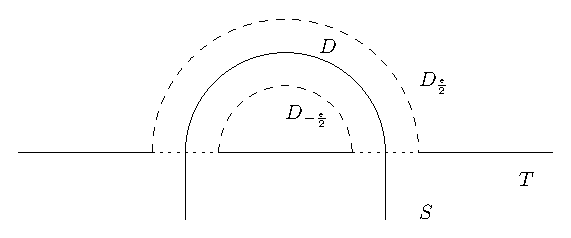
\includegraphics[width=0.54\textwidth]{surgery}
                \caption{Ausschneiden einer Umgebung von $S\cap T$ und Ankleben zweier Scheiben, sodass die Homologieklasse erhalten bleibt}
                \label{fig:surgery}
            \end{wrapfigure}
            Angenomme es existiert so ein Nullbordismus $D\subset S$ einer solchen Komponente $\partial D \subset S \cap T$. Weiter sei dieser auf dem Inneren disjunkt von $T$, da ein nichttrivialer Schnitt mit $T$ einen weiteren Kreis aus $S\cap T$ liefert, der den Nullbordismus einschränkt, sodass er weniger Komponenten im Schnitt mit $T$ berührt hat als der ursprüngliche (man bemerke das Transversalität genutzt wurde). So fahre man endlich oft fort, bis der Durchschnitt trivial ist beziehungsweise die berandende Scheibe, $T$ nur im Rand berührt.
            Nun lässt sich eine hinreichend kleine offene Tubenumgebung von $\partial D$ aus $T$ entfernen. Diese kann wie folgt gewählt werden: sei $\nu(S) \to M$ eine Tubenumgebung von $S$ die sich aufgrund der Zweiseitigkeit wie folgt wählen lässt: $\alpha: S \times (-\epsilon,\epsilon) \to M$, sodass $\im\alpha|_{S\times (-\frac 12\epsilon,\frac 12 \epsilon)} \cap T$ eine Tubenumgebung von $S\cap T \subset T$ ist. Dann lässt sich diese Tubenumgebung bei $\partial D$ aus $T$ entfernen und mittels der Zweiseitigkeit um $D$, findet man zwei Kopien $D_{\frac \epsilon 2}, D_{-\frac \epsilon 2}$, sowie Anklebevorschriften, mit denen diese Scheiben an die beiden durch Ausschneiden entstandenden Kreis-Randkomponenten kleben kann, vergleiche Abbildung~\ref{fig:surgery}. Als Resultat ergeben sich Flächen $S,T'$, deren Durchschnitt um eine Komponente reduziert wurde und offensichtlich $[T]=[T']$ gilt. \todo{kein Weg aus dem Durchschnitt ist rel Endpunkt homotop zu einem Rand}

            Von nun an seien $S,T$ transversale Flächen, deren Durchschnitt den obigen Anforderungen genügt. Ziel ist es nun, den Zykel, der die Vereinigung repräsentiert, als eingebettete Fläche zu repräsentieren. Beachtet man die Orientierungen, so kann man an jeder Komponente des Durchschnitts die Vereinigung aufschneiden (die lokal aussieht wie die Gerade an der sich zwei orientierte Ebenen im $\RR^3$ schneiden), und entlang der Orientierungen in nur einer Möglichkeit wieder verkleben, so dass man eine Mannigfaltigkeit erhält (dies funktioniert offensichtlich an den Durchschnittkomponenten mit Rand, aber auch den den geschlossenen Komponenten, da die Orientierungen auf $S$ und $T$ global gewählt sind). Natürlich können mit entsprechenden Umgebungen, alle diese Klebe- und Schneideprozesse glatt durchgeführt werden. Nun erhält man eine glatte, orientierte Fläche $U$, die (nach gegebenfalls leichter Modifikation) auch eigentlich eingebettet ist. Nun muss dieses Ergebnis und die Auswirkungen der Konstruktionen auf die Flächen diskutiert werden. Die "`uneinschränkenden"' Konstruktionen zu Beginn, können natürlich die Euler Charakteristik verändern, jedoch resultieren daraus weiterhin Thurston-Norm minimierende Flächen\footnote{Dies geschieht zum Beipsiel durch die Entstehung von Sphären. Wichtig ist nur dass solche Komponenten nicht beim Verkleben der beiden Flächen entstehen. Genau deswegen wurde diese Annahme getroffen.}. Zwei \emph{solche} Flächen gegeben, erbt die letztere Konstruktion, die aus $S\cup T$ eine homologe Fläche $U$ macht, die Summe der Eulercharakteristika:
            \begin{eqnarray*}
                \chi(U) = \chi(S) + \chi(T) &\implies& \chi_-(U)=\chi_-(S) + \chi_-(T) 
            \end{eqnarray*}
            wobei die Implikation gilt, da bei der Konstruktion von $U$ keine Komponenten mit positiver Eulercharakterstik entstehen, unter den an $S$ und $T$ gestellten Annahmen. Dies liefert nun die Subbadditivität der Thurston-Norm auf den Homologieklassen.
        \qed
        \vspace{6pt}

        Häufig stellt man Annahmen an die 3-Mannigfaltikeit, die es verbieten, dass Homologieklassen von Sphären oder Tori repräsentiert werden können. In dem Fall würde dann sogar $||\phi||_T=0 \Leftrightarrow \phi=0$ gelten. Dies alles motiviert natürlich, diese Norm zu einer Vektorraumnorm auf $H^1(M;\QQ)$ oder $H^1(M;\RR)$ fortzusetzen. 
        \begin{bem}[Fortsetzung von $||\cdot||_T$]
        \label{rem:extendingthurston}
            Will man $||\cdot||_T: H^1(M;\ZZ) \to \RR$ fortsetzen, so hilft die in Lemma~\ref{lem:norm} gezeigte Skalarmultiplikativität. Da $H^1(M;\ZZ)$ als $\ZZ$-Modul frei mit Rang $n$ ist, liefert die Einbettung $\ZZ^n \into \QQ^n$ zusammen mit der Linearität der Thurston-Norm eine lineare Fortsetzung auf den Strahlen (1-dimensionale Untervektorräume), die von Gitterpunkten erzeugt werden. Da aber für jedes $q \in \QQ^n$, bereits $aq \in \ZZ^n$ gilt (für großes $a\in \ZZ$), liefert dies bereits eine Fortsetzung auf $H^1(M;\QQ)$. Nun ist aber diese Fortsetzung mit Lemma~\ref{lem:norm} eine Halbnorm, insbesondere eine konvexe Funktion, also auf jedem Kompaktum Lipschitz-stetig und somit auf jedem Kompaktum $K\cap \QQ^n, K\subset \RR^n$ in eindeutiger Weise stetig auf $K$ fortsetzbar --- es folgt die Existenz von $||\cdot||_T:H^1(M;\RR) \to \RR$.
        \end{bem}
        Nun stehen die Definitionen der Invarianten bereit, die auf den folgenden Seiten untersucht werden sollen.
